%%%%%%%%%%%%%%%%%%%%%%%%%%%%%%%%%%%%%%%%%%%%%%%%%%%%%%%%%%%%%%%%%%%
%% chapter1.tex
%% UNL thesis document file
%%
%% Chapter with introduction
%%%%%%%%%%%%%%%%%%%%%%%%%%%%%%%%%%%%%%%%%%%%%%%%%%%%%%%%%%%%%%%%%%%
\newcommand{\unlthesis}{\emph{unlthesis}}
\newcommand{\unlthesisclass}{\texttt{unlthesis.cls}}


\chapter{Introduction}
\label{cha:introduction}

\section{Context}

Although during conversations major attention is given to the spoken content, non-verbal communication processing occurs subconsciously. Besides the verbal content of speech, it contains also non-verbal elements known as paralanguage: voice quality, rate, pitch, volume, and speaking style, prosodic features such as rhythm, intonation, and stress. But there are additional visual cues part of the non-verbal communication, namely, body language (kinesics), distance (proxemics), oculesics (eye contact, patterns of fixation, etc.), and touch (haptics). Together with paralanguage, non-verbal communication make two thirds of communication \cite{Burgoon2016}.

As such an important part of communication is visual, the goal of this thesis is to collect RGB and depth video data related to communication, analyze and detect different communication features by applying image processing techniques as well as machine learning. For that purpose different study cases have been carefully selected:
\begin{enumerate}
    \item \textbf{Speech and Language Therapy}: evaluation of oromotoric exercises performed by children with lisp problems in context of the project BioVisualSpeech.
    \item \textbf{Affective computing}: detecting and recognizing emotional states of humans.
    \item \textbf{Facial paralysis}: detect and quantify the severity of facial paralysis \cite{Ngo2016}\cite{Sundaraj2012}.
\end{enumerate}

Study case 1) is part of an international project called BioVisualSpeech in which this thesis is part of. In Fig.\ref{fig:project} an overview of the project, which aims to collect data from children with speech disorders, is provided. The project is composed by three main components: a) data acquisition using interactive games, b) Data analysis, and c) health information system. The goal of BioVisualSpeech is to develop a system that is composed by the three mentioned components in order to support speech therapists (more details in chapter \ref{sec:motivation}). During this thesis the focus lies on RGB and depth video processing, annotation extraction and development of a system which uses machine learning techniques to find similar patients and suggest therapy exercises. 

\begin{figure}
    \centering
    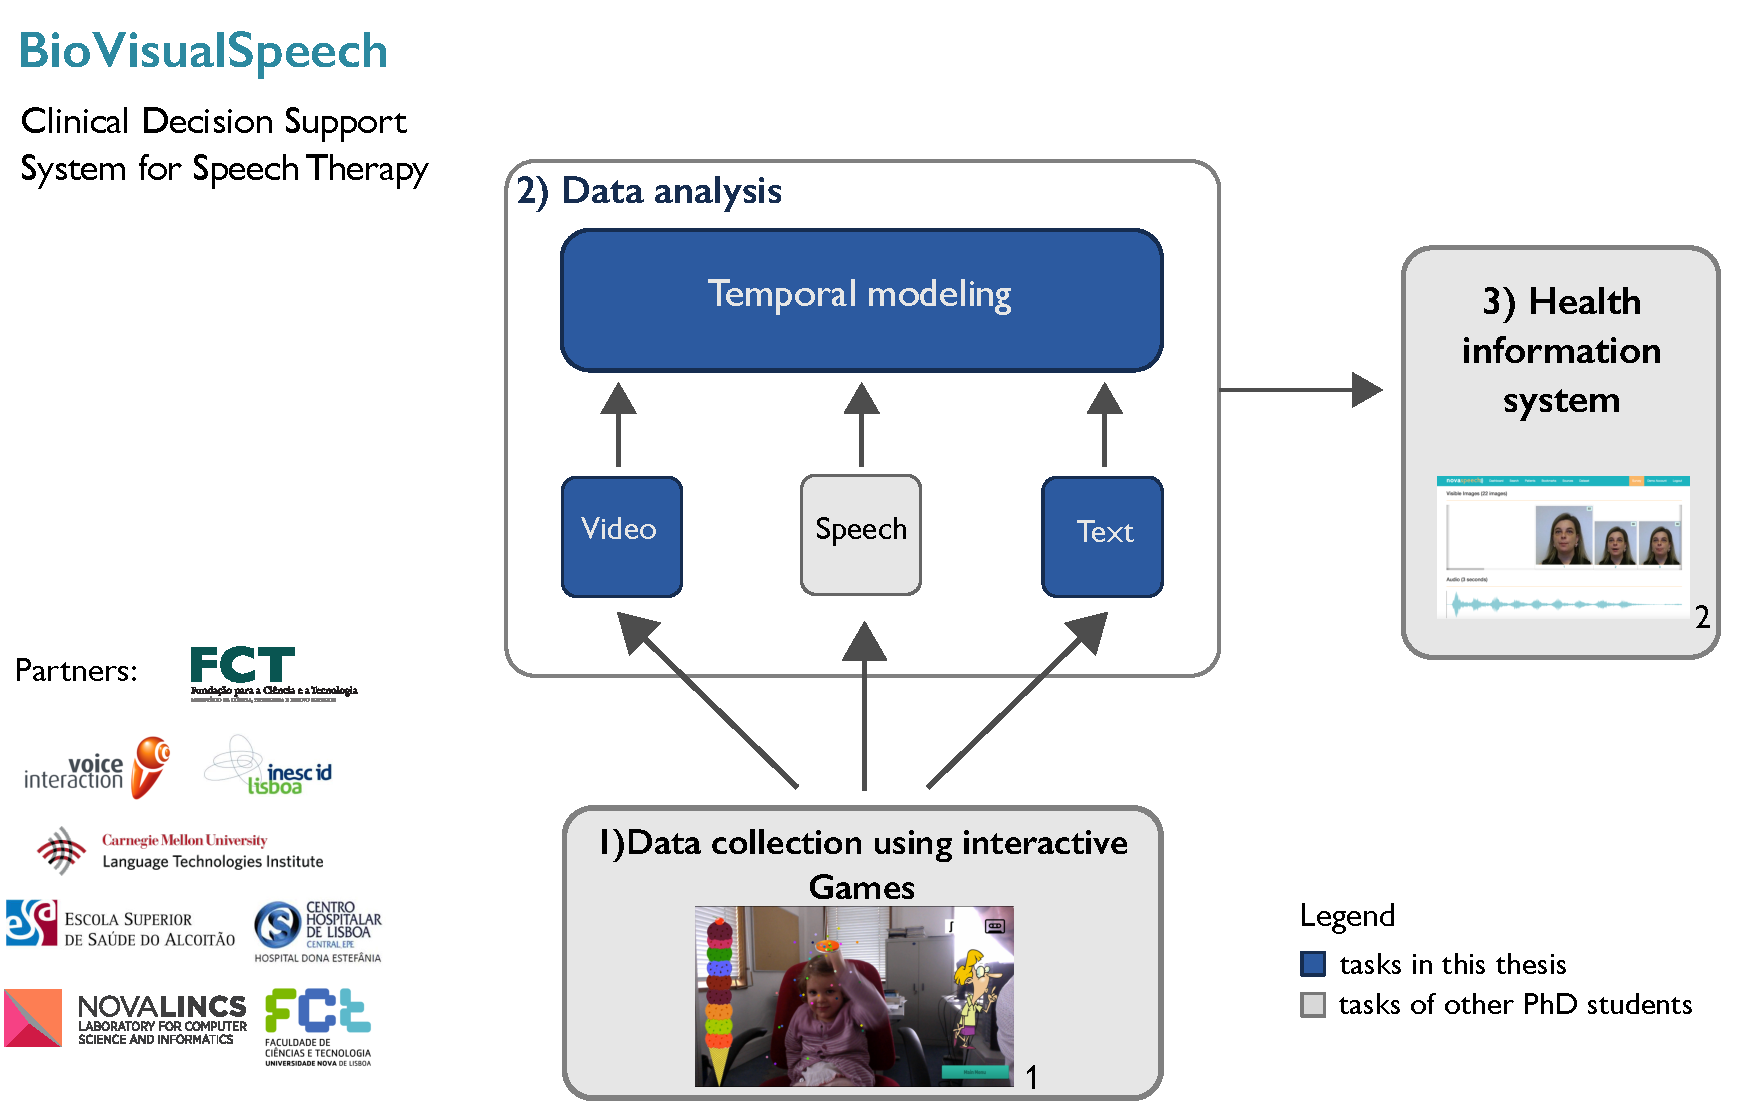
\includegraphics[width=13cm]{diagramProject.pdf}
    \caption{Overview of the project BioVisualSpeech.}
    \label{fig:project}
\end{figure}

Study case 2) was chosen as several datasets for expression detection are available and a taxonomy for facial movements is available in this area. As in study case 1) also facial movements have to be extracted and represented, the goal is to learn the state-of-the-art in expression detection in order to apply it to study case 1).

Study case 3) is similar to study case 1) with the difference that there is no pathology concerning speech. However, neurological diseases can cause facial paralysis which are visible and which disturb speech production and non-verbal communication. Through physiotherapy during several weeks, the gravity of the paralysis can be reduced. 

All three study cases have in common the video analysis of facial activity over a temporal window and it is expected that the same image processing and machine learning tools can be applied. In the following subchapters the motivation and impact will be described.  



% ==================================================================

\section{Motivation} % (fold)
\label{sec:motivation}

The human face can provide several insights such as the emotional state, symptoms of diseases (pain, elevated blood pressure, facial paralysis, autism etc.), engagement in a conversation, and so on. However, the given examples are difficult to measure quantitatively and are mainly subjective.\\

In 1995, Rosalind Picard first published the term affective computing which has become a growing interdisciplinary research area in the last years. The area started by the curiosity to measure the emotional state of study participants quantitatively instead of being measured by questionnaires through self-reporting \cite{Picard2014promise}. Detection and understanding of human affects have become important not only in human-computer interaction but also in areas such as medicine, literature, psychology, and marketing.\\

Such as the human face musculature is important to express feelings and the interior state of mind, it is also essential for verbal communication. Understanding facial activity during speech could help improve speech analysis when speech recording has poor quality or is not present. Additionaly, by knowing how facial muscles are engaged during speech, dysfunction and its severity could be detected. Understanding the tools used for facial expression detection in order to apply them to health domains such as speech therapy is one of the main goals of this thesis.

And why speech therapy? In the year 2000, 40 million Americans had communication disorders causing a cost to the U.S. of approximately \$154-186 billion anually which was equal to 2.5-3\% of the Gross National Product \cite{Ruben2000}. The U.S. employment market has become more and more dependent on communication skills (hearing, voice, speech, and language) as in several industries manual work is being automated. And although it might seem that hearing loss brings more economic disadvantage than the lack of another communication skill, people with severe speech disabilities are more often unemployed or in a lower economic class \cite{Ruben2000}.

In order to reduce prevalence of speech disorders, it is essential to detect and treat speech disabilities as soon as possible, considering that 5\% of US children aged 3-17 years have a  speech disorder, which means that they have difficulties in producing sounds of speech and problems with the quality of voice \cite{SpeechStatistics}. Supporting speech and language therapists (SLTs) in that task is the purpose of the project BioVisualSpeech. The goal of this project is to develop a system that provides SLTs with exercises incorporated in interactive games and an information system that enables therapists to easily review the exercise performance of their patients through video recordings. The main goal however, is to develop a machine learning system that analyzes the data collected during the games and recognizes patterns using data of other patients in order to extract new insights and suggest exercises that suit the learning progress of the patient.  

The same setting could also be applied to patients with facial paralysis, caused by nerve damage. It usually occurs on only one side of the face and can have different degrees of severity which cause difficulty not only in speaking but also in eating and drinking. Although there are more than twenty grading methods of the severity of facial paralysis, they have defaults in integration, feasibility, accuracy, and reliability \cite{Dong2008}. The development of an accurate method for detection and grading of facial paralysis based on image processing would be beneficial to clinicians and patients.


For both, speech therapy and facial paralysis therapy, treatment takes several months of therapy sessions in which various exercises are performed to improve weakness in oral musculature. The video monitoring during therapy combined with the analysis of face muscle performance could help therapists to follow up the progress of each patient, compare patients with similar problems and even provide therapists with quantitative measurements. The inclusion of affective computing in the face analysis system, would accquire additional information of the patient's degree of engagement during the exercises being an additional factor to a successful therapy. Through the use of different sources of data such as health records, a multimodal time series of observations is used to develop a clinical decision support system that supports therapists in providing personalized therapies.
% ==================================================================

\section{Challenges and Impact}

\begin{itemize}
    \item What are the difficulties that you wish to overcome?
    \item If you overcome them what impact would it produce in the real-world? (patients? health professionals?)
\end{itemize}

\textbf{Challenge 1. Understanding human face muscles}
The human face is composed by 43 muscles. Without them we would be missing an important tool for communicating not only with people from our cultural environment but also with people from different provenience as the only way to be understood would be through gestures. Our facial muscles are essential for both, verbal and non-verbal communication.\par 
For verbal communication besides tongue, larynx, pharynx, and soft palate muscles, which are not visible from the exterior, also lip and mandibular muscles are crucial (orbicularis oris: close lips, levator labii superioris: raise upper lip, more in \cite{PhonManual}). 
Malfunction of these muscles can be caused by neurological or motoric problems. Examples for the first cause are brain stroke and Bell's Palsy which cause facial paralysis.

overview of muscles and importance
the use of them during speech
problems that exist in speech therapy
necessity of solving this problem

2) image processing given data recorded in different conditions (light, position, children (smaller head), head position). Complexity of human communication (many combinations of action units).\\


----Thoughts 20.04.17:\\
\textbf{Challenge 2. Representation of different modalities and temporal information}

Find a fitting feature space. \\


Impact 1) provide an additional tool to therapists that enables them to take advantage of data collected from other patients. By using insights of the data, actions that are beneficial to the therapy for specific patients can be detected $\rightarrow$ personalized therapy.\\
2) impact of emotional state of the patient can be taken into account and explain fast/slow progress.\\
3) save therapists time, help them predict therapy length\\
4) patients have a tailored therapy given on continuously obtained new insights\\ 
!use instead of therapist, health professionals (check definition)
----\\
% ==================================================================


\section{Scope and Objectives}

\begin{itemize}
    \item in one sentence (3 lines) describe the goal of your thesis in a way that ``everyone'' understands
    \item formulate a research hypothesis for the specialist audience. What is your idea?
\end{itemize}


Considering clinical medical data existing in the Electronic Health Records, in particular, multimodal time series of data from health sensors and medical notes collected at each patient visit, we wish to recognize health/clinical patterns to support health professionals in their decisions through (i) suggestions and (ii) similar examples.

----Thoughts 20.04.17:\\
my work will focus on image processing, specifically using video recordings. My interest lies in detecting facial activity which maybe caused during speech or just  by emotions. I want to detect if a person has difficulties in articulation which are caused by motoric dysfunctions of speech. But also want to analyze non-verbal communication triggered by emotions (disengagement of patient in the therapy, fatigue). I want to map facial muscle activity which is visible to correct/incorrect execution of speech exercises; map to different emotions and intensity. Understand two types of communication: 1) physical and visible characteristics of speech production, 2) non-verbal communication.\\

To map facial activity for both communications I need to experiment different feature representations in different feature spaces. Might be that for each type of communication a separate feature space is needed. Will test if mapping improves by including additional data from different modalities, such as, speech and text annotations. \\

Another goal is to develop a model to include temporal information in the feature space. For that I will take the different data representations/embeddings as input for the temporal modelling. Develop mathematical model.\\

Goal is to apply this system to applications in which time has an important role, for example, in therapies (speech, psychology, etc.). Applications where temporal progression of a disease is observed through several therapy sessions.\\

By being able to model the temporal progress of therapy, the progress of one patient can be compared to other patients. Patients who had a similar starting point and who had a positive outcome of the therapy, can be taken as example and provide insights of therapeutic actions that can help other similar patients to improve their progress. Thus, future actions to take can be suggested to the therapist.   
\\
----\\

----Thoughts 20.04.17:\\
Develop multimodal feature space which includes temporal information. Testing of different embeddings. Create statistical model which permits suggesting future therapy sessions, by comparing one patient with similar ones in an existing database.\\
Understanding facial activity associated to non-verbal communication and to speech.\\ include diagram as scope and in that context say what the objective is.
----\\
research hypothesis not yet in CAT but later: writing of hypotheses write something no one did before, find niche that nobody tackled yet. 

\section{Contributions}

Contribution 1) A new dataset for 3D video dataset for oro-facial motor exercises with children.

Contribution 2) Benchmark of embeddings for facial representation.

Contribution 3) Survey of...


